\section{Future}

\subsection{Expected Results} \label{sec:ExpRes}

The most important aspects of the project that can be studied as being considered to be critical are:

\begin{itemize}
    \item Compactness (maximal average density of radiators achievable without isostatic compression)
    \item New and denser composite radiator materials
    \item Ultimate homogeneity
    \item Ultimate plastic fiber ratio
    \item Isostatically compressed Tungsten powder radiators
\end{itemize}

The first samples of Tungsten powder radiators (not sintered) with holes for fibers have been built at JLab by Cold Isostatic Pressing (CIP) at 150,000 psi (see Figure \ref{fig:Samples}).

\begin{figure}[h]
\centering
\includegraphics[width=0.975\linewidth]{images/Figure14_Samples_Crop.jpg}
\caption{Samples of isostatically compressed Tungsten powder prototype radiators.}
\label{fig:Samples}
\end{figure}

The density achieved with isostatic compression was 16.33 g/cm$^3$ i.e. 84.8\% of bulk Tungsten density. Our setup did not allow us to compress powder samples which already contained fibers without compromising the integrity of the sample (see Figure \ref{fig:CompressFibersIn}). Therefore we have addressed the above mentioned technical problem in order to reach ultimate average density of the powder radiator (see Section \ref{section:possibleImprovements}).

\begin{figure}[h]
\centering
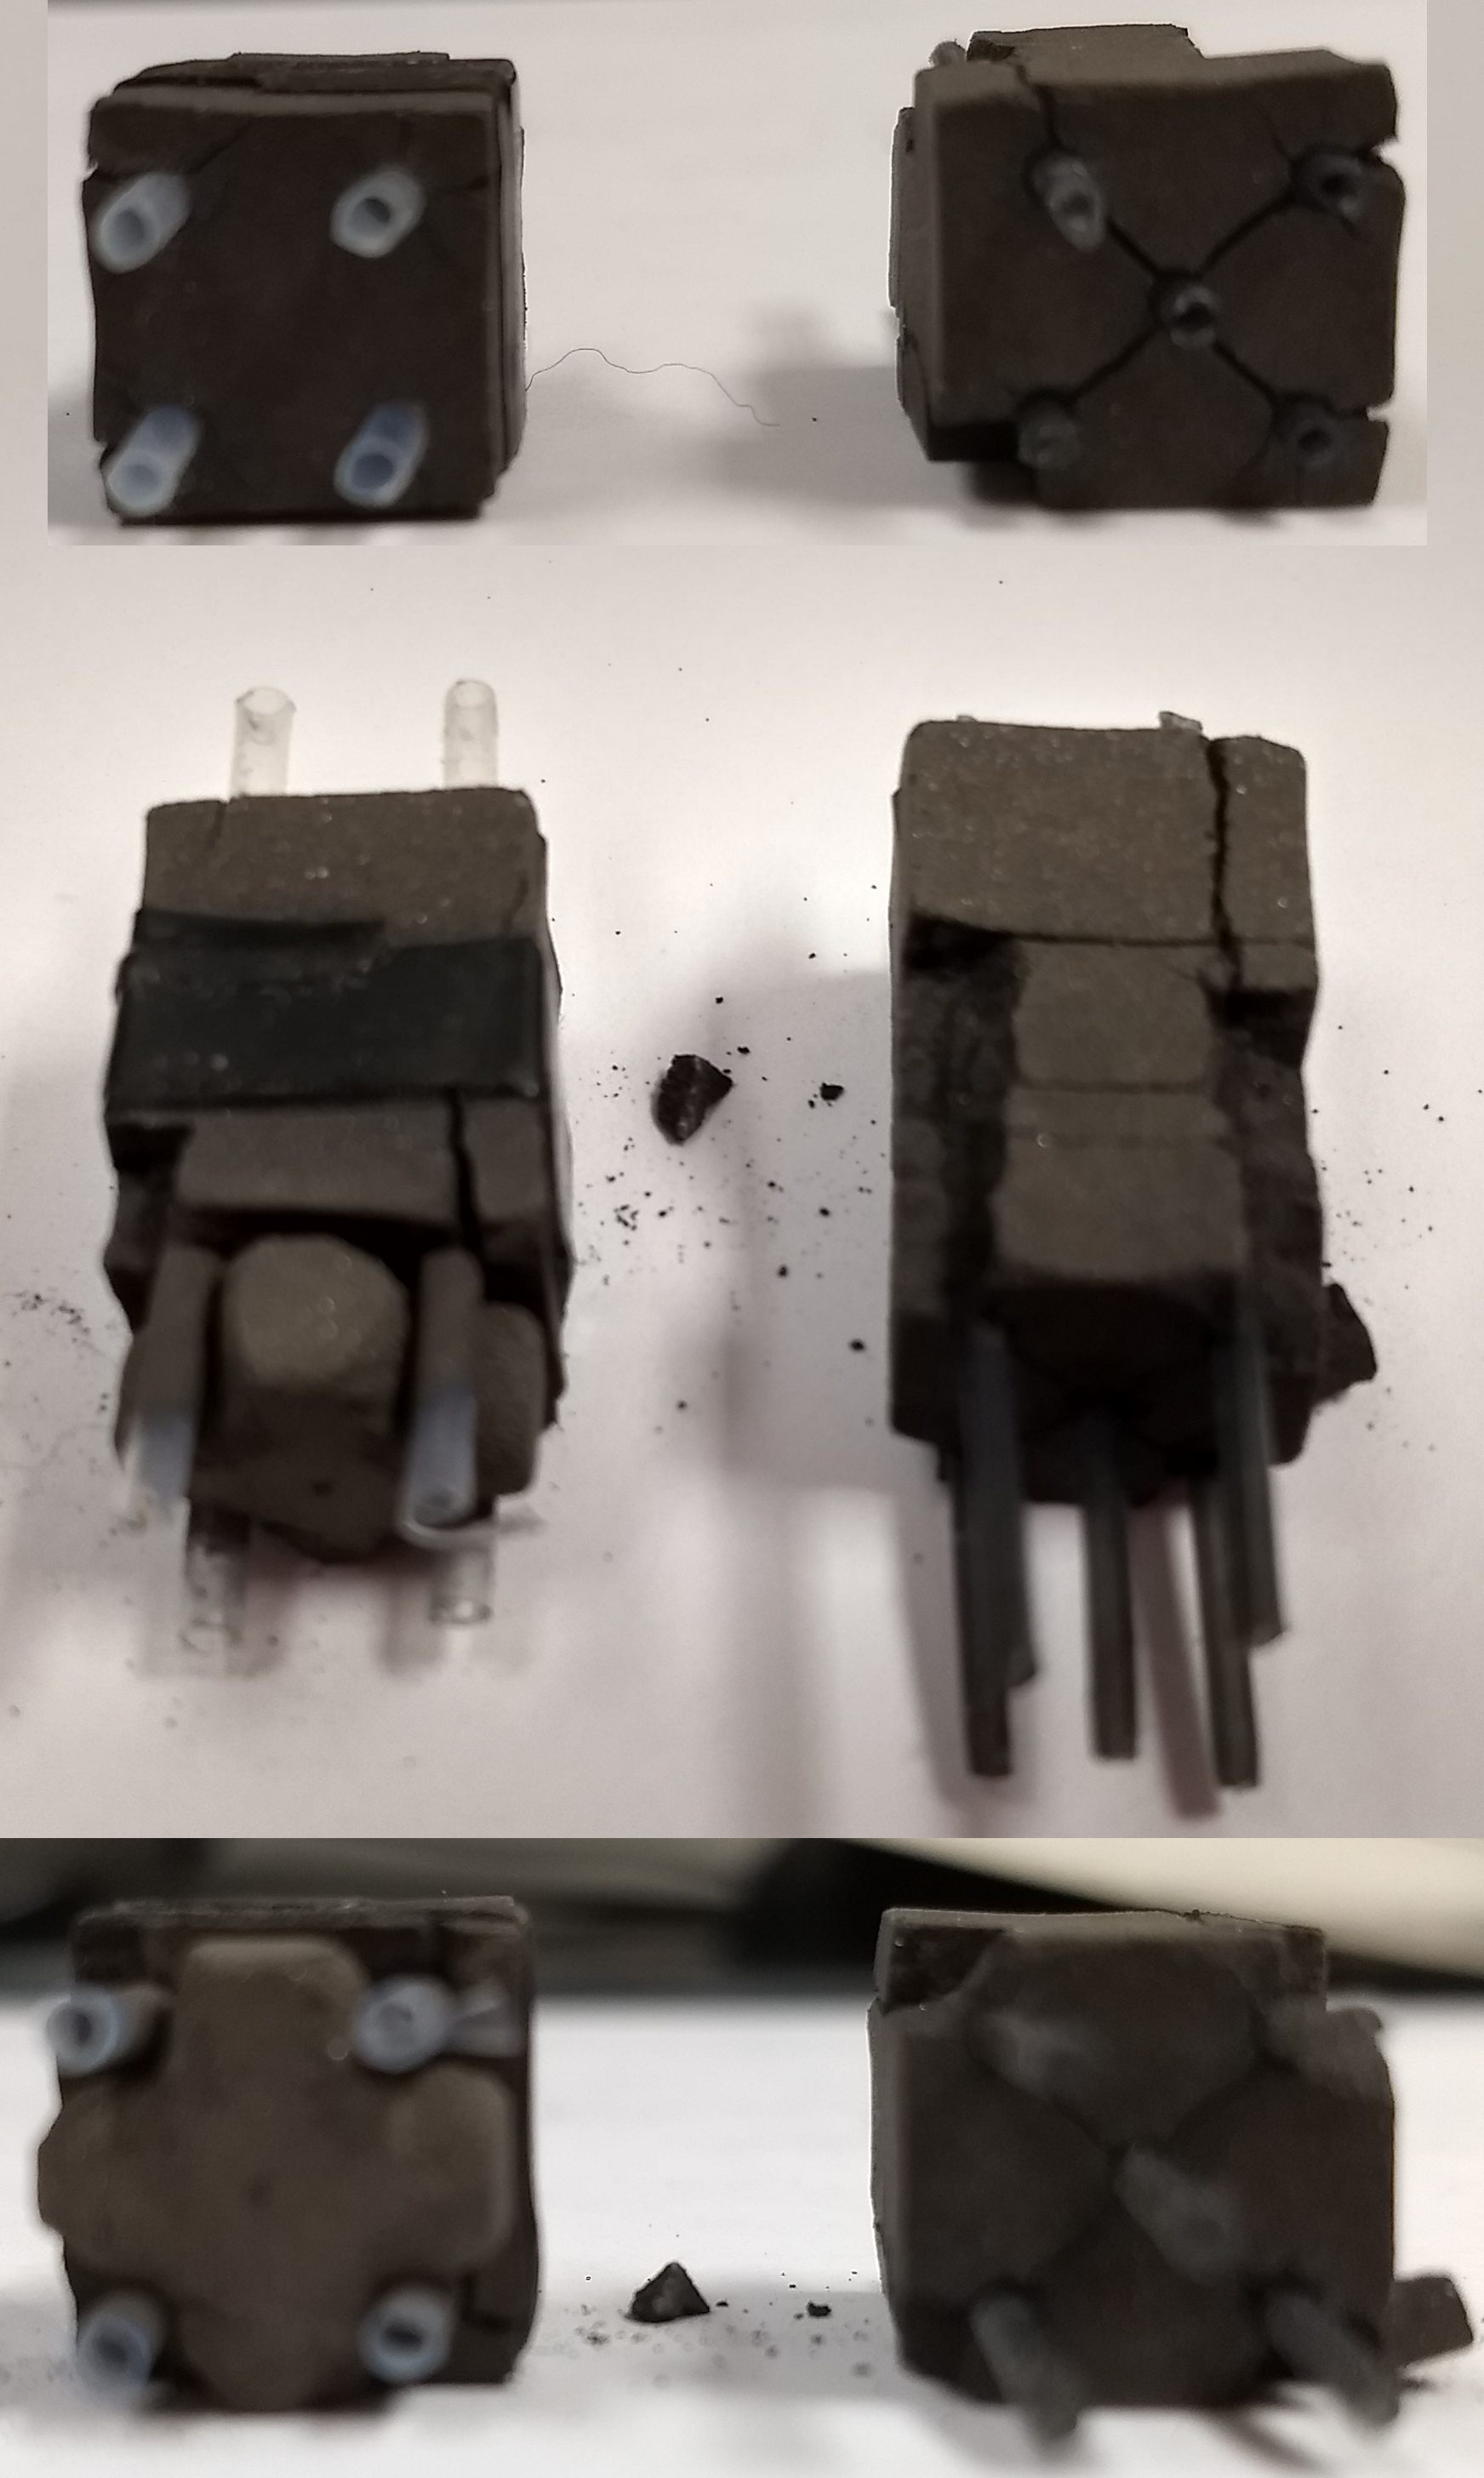
\includegraphics[width=0.9\linewidth]{images/Fig15_CompressFibersIn.png}
\caption{Two Tungsten powder prototype radiators that were compressed with fibers already embedded in them.}
\label{fig:CompressFibersIn}
\end{figure}

\subsection{Possible Improvements} \label{section:possibleImprovements}

In Section \ref{sec:ExpRes} we mention that via CIP we can obtain a Tungsten powder radiator with a density of 16.33 g/cm$^3$. Some issues of the CIP method are a result of the difficulty in creating the set-up itself, and in maintaining the integrity of the radiators. The problems arise if the fibers are already installed in the powder before the volume is isostatically compressed. During the compression the fibers as being liquid shrink considerably. At pressures we generated water, for instance, will be compressed by about 20\%. And when the radiator is removed the fibers then expand back to resume their original volume. This expansion causes destructive cracks in the radiators, which can be seen in Figure \ref{fig:CompressFibersIn}. Therefore we developed and tested alternative ways while still been using the cold isostatic compression technique to build high density powder radiators (84.8\% of the bulk Tungsten density). 

We used thin wall hypodermic stainless steel tubing installed in a sample powder radiator instead of fibers. In this case the tubes will be compressed both from outside and inside compensating each other. Since tubes have small wall thickness than compression of walls is even smaller if any. Probably the best results can be achieved with tubing of smallest possible wall thickness. 

\begin{figure}[h]
\centering
\includegraphics[width=0.975\linewidth]{images/Pwd_ss_tubes.png}
\caption{Isostatically compressed Tungsten powder sample radiator with hypodermic stainless tubing.}
\label{fig:Isostatic}
\end{figure}

Once compression process was completed the sample was left untouched and after certain time period when mechanical stresses were gone the stainless tubing have been removed (see Figure \ref{fig:Samples}). No special tools or procedures to follow were used. The inside surfaces of the holes in the sample radiator were as smooth as outside surface of the stainless tubing.Of course it was possible to leave the tubing not removed and use the radiator as is.
The cladded fibers put in the sample radiator undamaged and also without any damages caused to the radiator would unavoidably leave some unwanted air gaps. We have addressed this problem by running some tests with fibers to change their dimensions. 
In our tests we used 3mm thick and about 100cm long polystyrene fiber optics with acrylic cladding. Both ends of fiber were fixed in holders so that it was not completely stretched, i.e. it was hanging slightly loose. Then the entire setup was put into the high precision oven and then slow heating process was started. At temperatures bellow  $\sim$80\degree C the fiber would expend and get visible longer. At higher temperatures the fiber eventually becomes liquid of high viscosity. It would shrink to minimize its surface area due to surface tension forces. At temperatures $\sim$102-105\degree C the fiber got fully contracted and therefore stretched as a string between holders. Consequently its diameter was increasing depending on distance between holders and length of the fiber before heating. At this point we were gradually moving holders toward each other while maintaining temperature unchanged. The fiber shrank further. At the end we gradually cooled the fiber to room temperature. We have successfully obtained a very straight and perfectly round fiber with no defects on it that  had final diameter of 6mm. In other words one should expect having no gaps around fibers installed in the radiator using procedures described above.

At present, the final density of the Tungsten powder radiator is about 12 g/cm$^3$, and it could be possible be increased using CIP and reach higher densities up to 16.33 g/cm$^3$).    